% !TeX program = pdflatex

\documentclass[a4paper,12pt]{article}
% Сборка через pdfLaTeX.
\usepackage{cmap}
\usepackage[T2A]{fontenc}
\usepackage[utf8]{inputenc}
\usepackage[english,russian]{babel}
\usepackage{lmodern}
\usepackage{amsmath,amssymb}
\usepackage{geometry}
\geometry{left=22mm,right=18mm,top=20mm,bottom=20mm}
\usepackage{booktabs,longtable,array,multirow}
\usepackage{graphicx}
\usepackage{float}
\usepackage{caption}
\usepackage{pgfplots}
\usepackage{pgfplotstable}
\pgfplotsset{compat=1.18}
\usepackage{siunitx}
\sisetup{output-decimal-marker={,}, per-mode=symbol}
\usepackage{enumitem}
\setlist{nosep}
\usepackage{indentfirst}
\usepackage{hyperref}
\hypersetup{hidelinks}

\newcommand{\placeholder}[2]{%
\begin{figure}[H]
\centering
\fbox{\begin{minipage}[c][#1][c]{0.86\linewidth}\centering\vspace{2mm}#2\vspace{2mm}\end{minipage}}
\end{figure}}
\newcommand{\dd}{\,\mathrm{d}}
\newcommand{\eps}{\varepsilon}

\title{Отчет по лабораторной работе 2.2.3 \\ ИЗМЕРЕНИЕ ТЕПЛОПРОВОДНОСТИ
ВОЗДУХА ПРИ АТМОСФЕРНОМ
ДАВЛЕНИИ }
\author{Максим Осипов, Б03-504}
\date{\today}

\begin{document}
\maketitle

\section*{Аннотация}
В работе определён коэффициент теплопроводности воздуха при атмосферном давлении в диапазоне температур термостата от $22^\circ\mathrm{C}$ до $80^\circ\mathrm{C}$. Метод основан на измерении нагрузочных кривых $R_{\text{н}}(Q)$ металлической нити, расположенной вдоль оси цилиндрической колбы. По экстраполяции $Q\to 0$ получена температурная зависимость сопротивления нити
\[
R_0(\theta)=(19{,}230\pm 0{,}022)+(0{,}07184\pm 0{,}00039)\theta\quad [\Omega],
\]
где $\theta$ измеряется в $^\circ\mathrm{C}$. Получены значения $\kappa=(28{,}43\pm0{,}54)\ldots(35{,}15\pm1{,}20)\,\text{мВт}/(\text{м}\cdot\text{К})$. Аппроксимация $\kappa\propto T^{\beta}$ дала показатель
\[
\beta=1{,}09\pm 0{,}17.
\]

\section{Теория}

\subsection{Закон Фурье и кинетическая оценка теплопроводности}
Теплопроводность --- перенос энергии от более нагретых областей к более холодным за счёт хаотического движения частиц. В локально равновесном состоянии плотность теплового потока $\vec q$ пропорциональна градиенту температуры:
\begin{equation}
\vec q=-\kappa\nabla T.
\label{eq:fourier}
\end{equation}
Знак минус показывает, что тепло течёт в сторону убывания температуры. Размерность $\kappa$ следует из $[q]=\text{Вт}/\text{м}^2$ и $[\nabla T]=\text{К}/\text{м}$:
\[
[\kappa]=\frac{\text{Вт}/\text{м}^2}{\text{К}/\text{м}}=\text{Вт}/(\text{м}\cdot\text{К}).
\]

Кинетическая оценка получается следующим образом. Молекула, прошедшая перед столкновением путь порядка длины свободного пробега $\lambda$, переносит энергию, характерную для температуры той области, из которой она пришла. При изменении температуры на расстоянии $\lambda$ разность энергий одной молекулы порядка
\[
\Delta \eps\sim c_V\Delta T\sim c_V\lambda |\nabla T|,
\]
где $c_V$ --- теплоёмкость одной молекулы при постоянном объёме. За единицу времени через единичную площадку проходят молекулы с потоком порядка $n\overline v$, поэтому
\[
q\sim n\overline v\,c_V\lambda |\nabla T|.
\]
Сравнивая это выражение с законом Фурье \eqref{eq:fourier}, получаем оценку
\begin{equation}
\kappa\sim \lambda \overline v n c_V.
\label{eq:kappa_mkt}
\end{equation}
Для идеального газа $c_V=(i/2)k_{\mathrm B}$, а средняя тепловая скорость молекул
\[
\overline v=\sqrt{\frac{8k_{\mathrm B}T}{\pi m}}.
\]
Если длина свободного пробега оценивается как
\[
\lambda\sim\frac{1}{n\sigma},
\]
где $\sigma$ --- эффективное сечение столкновений, то
\[
\kappa\sim \frac{\overline v c_V}{\sigma}.
\]
Отсюда видно, что при фиксированном составе газа теплопроводность слабо зависит от давления: множитель $n$ сокращается с $\lambda\sim 1/n$. В модели твёрдых шариков $\sigma=\mathrm{const}$, следовательно,
\begin{equation}
\kappa\propto \overline v\propto \sqrt{T}.
\label{eq:hard_spheres}
\end{equation}

\subsection{Теплопередача в цилиндрической геометрии}
Рассматривается длинный цилиндр радиуса $r_0$, вдоль оси которого натянута тонкая нить радиуса $r_1$ и длины $L$. Температура стенок поддерживается равной $T_0$, температура нити равна $T_1$, перегрев нити
\[
\Delta T=T_1-T_0.
\]
При $L\gg r_0$ теплоотводом через торцы можно пренебречь, а тепловой поток считать радиальным. Тогда из \eqref{eq:fourier}
\begin{equation}
q_r=-\kappa\frac{\dd T}{\dd r}.
\label{eq:radial_fourier}
\end{equation}
Площадь цилиндрической поверхности радиуса $r$ равна
\[
S(r)=2\pi rL.
\]
Полная мощность, проходящая через эту поверхность, одинакова для любого $r$:
\begin{equation}
Q=q_rS(r)=-2\pi rL\kappa\frac{\dd T}{\dd r}=\mathrm{const}.
\label{eq:flow_constant}
\end{equation}
Выразим дифференциал температуры:
\[
\frac{\dd T}{\dd r}=-\frac{Q}{2\pi L\kappa}\frac{1}{r},
\qquad
\dd T=-\frac{Q}{2\pi L\kappa}\frac{\dd r}{r}.
\]
При малом перегреве $\Delta T\ll T_0$ коэффициент $\kappa$ в пределах газового слоя можно считать постоянным и равным $\kappa(T_0)$. Интегрируем от поверхности нити до стенки:
\[
\int_{T_1}^{T_0}\dd T=-\frac{Q}{2\pi L\kappa}\int_{r_1}^{r_0}\frac{\dd r}{r}.
\]
Левая часть равна $T_0-T_1=-\Delta T$, правая часть равна
\[
-\frac{Q}{2\pi L\kappa}\ln\frac{r_0}{r_1}.
\]
Следовательно,
\[
-\Delta T=-\frac{Q}{2\pi L\kappa}\ln\frac{r_0}{r_1},
\qquad
\Delta T=\frac{Q}{2\pi L\kappa}\ln\frac{r_0}{r_1}.
\]
Отсюда основная расчётная формула:
\begin{equation}
Q=\frac{2\pi L\kappa}{\ln(r_0/r_1)}\Delta T,
\qquad
\kappa=\frac{\ln(r_0/r_1)}{2\pi L}\frac{Q}{\Delta T}.
\label{eq:main}
\end{equation}

\subsection{Нагрузочные кривые и термометр сопротивления}
В опыте металлическая нить одновременно служит нагревателем и термометром сопротивления. Измеряются напряжение $U$ и ток $I$; сопротивление и мощность находятся по формулам
\begin{equation}
R_{\text{н}}=\frac{U}{I},\qquad Q=UI.
\label{eq:RUQ}
\end{equation}
Если $U$ задано в мВ, а $I$ в мА, то
\[
R_{\text{н}}[\Omega]=\frac{U[\text{мВ}]}{I[\text{мА}]},
\qquad
Q[\text{мВт}]=\frac{U[\text{мВ}]\,I[\text{мА}]}{1000}.
\]
При фиксированной температуре стенок $T_0$ зависимость $R_{\text{н}}(Q)$ аппроксимируется прямой
\begin{equation}
R_{\text{н}}=R_0+aQ,
\label{eq:load_curve}
\end{equation}
где $R_0=R_{\text{н}}(0)$ --- сопротивление нити при отсутствии нагрева. При $Q\to0$ температура нити совпадает с температурой стенок, поэтому значения $R_0$ дают калибровку термометра сопротивления. В исследованном диапазоне температур используется линейная зависимость
\begin{equation}
R_0(t)=R_{273}(1+\alpha\ t)=R_{273}+bt,
\qquad b=\frac{\dd R}{\dd T}=\alpha R_{273},
\label{eq:RT}
\end{equation}
где $t$ --- температура в $^\circ\mathrm{C}$.

Свяжем наклон нагрузочной кривой с перегревом нити. Из \eqref{eq:RT}
\[
\Delta R=b\Delta T,
\]
а из \eqref{eq:load_curve}
\[
\Delta R=aQ.
\]
Исключая $\Delta R$, получаем
\[
aQ=b\Delta T,
\qquad
\frac{Q}{\Delta T}=\frac{b}{a}.
\]
Подстановка в \eqref{eq:main} даёт рабочую формулу
\begin{equation}
\boxed{\kappa_j=\frac{\ln(r_0/r_1)}{2\pi L}\frac{b}{a_j}},
\label{eq:kappa_working}
\end{equation}
где $a_j=(\dd R/\dd Q)_{T_0=T_j}$ --- наклон нагрузочной кривой при $j$-й температуре термостата.

\subsection{Оценка времени установления стационарного состояния}
Для слоя газа толщины $a$ тепловой поток по порядку величины равен
\[
q\sim \kappa\frac{\Delta T}{a}.
\]
За время $\tau$ через площадь $S$ поступит тепло
\[
Q_\tau\sim qS\tau\sim \kappa\frac{\Delta T}{a}S\tau.
\]
Для прогрева всего слоя на $\Delta T$ требуется тепло
\[
Q_C\sim n c_P Sa\Delta T.
\]
Приравнивая $Q_\tau$ и $Q_C$, получаем
\[
\kappa\frac{\Delta T}{a}S\tau=n c_P Sa\Delta T,
\qquad
\tau\sim\frac{a^2 n c_P}{\kappa}=\frac{a^2}{\chi},
\]
где
\begin{equation}
\chi=\frac{\kappa}{n c_P}
\label{eq:diffusivity}
\end{equation}
--- коэффициент температуропроводности.




\section{Результаты измерений}

\begin{figure}[h]
    \centering
    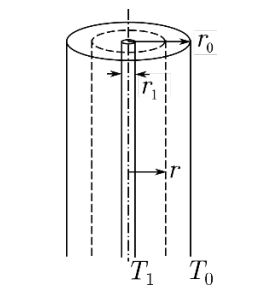
\includegraphics[width=0.3\textwidth]{геометрия.png}
    \caption{Геометрия задачи}
    \label{fig:lnU_45}
\end{figure}

\begin{figure}[h]
    \centering
    
\includegraphics[width=0.6\textwidth]{установка.png}
    \caption{Установка}
    \label{fig:lnU_45}
\end{figure}


Использованные при обработке геометрические параметры установки:
\begin{equation}
2r_0=(1{,}00\pm0{,}01)\,\text{см},\qquad
2r_1=(0{,}050\pm0{,}001)\,\text{мм},\qquad
L=(40{,}0\pm0{,}5)\,\text{см}.
\label{eq:geom_values}
\end{equation}
Отсюда
\[
\ln\frac{r_0}{r_1}=\ln\frac{5{,}0\cdot10^{-3}}{2{,}5\cdot10^{-5}}=\ln 200=5{,}298,
\]
\[
\gamma\equiv\frac{\ln(r_0/r_1)}{2\pi L}=\frac{5{,}298}{2\pi\cdot0{,}400}=2{,}108\,\text{м}^{-1},
\qquad
\frac{\sigma_\gamma}{\gamma}=1{,}32\%.
\]

Предельный перегрев при подготовительной оценке принят равным $\Delta T_{\max}=30\,\text{К}$, $\kappa\approx25\,\text{мВт}/(\text{м}\cdot\text{К})$. Тогда
\[
Q_{\max}=\frac{2\pi L\kappa}{\ln(r_0/r_1)}\Delta T_{\max}
=\frac{2\pi\cdot0{,}400\cdot25\cdot10^{-3}}{5{,}298}\cdot30=0{,}356\,\text{Вт}.
\]
При $R_{\text{н}}\approx21\,\Omega$
\[
I_{\max}=\sqrt{\frac{Q_{\max}}{R_{\text{н}}}}
=\sqrt{\frac{0{,}356}{21}}=0{,}130\,\text{А},
\qquad
U_{\max}=I_{\max}R_{\text{н}}=0{,}130\cdot21=2{,}73\,\text{В}.
\]

\subsection{Сведения о погрешностях прямых измерений}
Паспортные формулы точности мультиметров в исходных данных отсутствовали, поэтому при расчётах приняты погрешности отсчёта по младшему разряду записи и погрешность термостата:
\[
\sigma_U\simeq0{,}1\,\text{мВ},\qquad
\sigma_I\simeq0{,}01\text{--}0{,}1\,\text{мА},\qquad
\sigma_{T_0}\simeq0{,}5^\circ\mathrm{C}.
\]
Для косвенно найденных $R_{\text{н}}$ и $Q$ используются формулы распространения погрешностей
\begin{equation}
\sigma_R=R_{\text{н}}\sqrt{\left(\frac{\sigma_U}{U}\right)^2+\left(\frac{\sigma_I}{I}\right)^2},
\qquad
\sigma_Q=Q\sqrt{\left(\frac{\sigma_U}{U}\right)^2+\left(\frac{\sigma_I}{I}\right)^2}.
\label{eq:direct_uncertainties}
\end{equation}
Для итоговых коэффициентов прямых использовались стандартные ошибки линейной регрессии, так как они учитывают фактический разброс точек на нагрузочных кривых.

Пример обработки первой точки:
\[
R_{\text{н}}=\frac{229{,}8\,\text{мВ}}{11{,}03\,\text{мА}}=20{,}834\,\Omega,
\]
\[
Q=229{,}8\,\text{мВ}\cdot11{,}03\,\text{мА}=2534{,}7\,\text{мкВт}=2{,}535\,\text{мВт}.
\]

\begin{longtable}{ccccc}
\caption{Экспериментальные данные и рассчитанные по ним $R_{\text{н}}$ и $Q$.}\\
\toprule
$T_0,\ ^\circ\mathrm{C}$ & $U$, мВ & $I$, мА & $R_{\text{н}}$, $\Omega$ & $Q$, мВт \\
\midrule
\endfirsthead
\toprule
$T_0,\ ^\circ\mathrm{C}$ & $U$, мВ & $I$, мА & $R_{\text{н}}$, $\Omega$ & $Q$, мВт \\
\midrule
\endhead
22 & 229{,}8 & 11{,}03 & 20{,}834 & 2{,}535 \\
22 & 418{,}5 & 20{,}1 & 20{,}821 & 8{,}412 \\
22 & 631{,}3 & 30{,}2 & 20{,}904 & 19{,}065 \\
22 & 838{,}6 & 39{,}9 & 21{,}018 & 33{,}460 \\
22 & 1066{,}7 & 50{,}6 & 21{,}081 & 53{,}975 \\
22 & 1287{,}5 & 60{,}7 & 21{,}211 & 78{,}151 \\
22 & 1495{,}1 & 70{,}0 & 21{,}359 & 104{,}657 \\
22 & 1720{,}6 & 79{,}9 & 21{,}534 & 137{,}476 \\
22 & 1968{,}0 & 90{,}5 & 21{,}746 & 178{,}104 \\
22 & 2216{,}4 & 100{,}9 & 21{,}966 & 223{,}635 \\
22 & 2427{,}9 & 109{,}4 & 22{,}193 & 265{,}612 \\
22 & 2690{,}5 & 119{,}3 & 22{,}552 & 320{,}977 \\
37 & 2799{,}3 & 118{,}9 & 23{,}543 & 332{,}837 \\
37 & 2538{,}6 & 109{,}17 & 23{,}254 & 277{,}139 \\
37 & 2318{,}2 & 100{,}6 & 23{,}044 & 233{,}211 \\
37 & 2077{,}0 & 90{,}9 & 22{,}849 & 188{,}799 \\
37 & 1792{,}7 & 79{,}3 & 22{,}607 & 142{,}161 \\
37 & 1577{,}3 & 70{,}3 & 22{,}437 & 110{,}884 \\
37 & 1357{,}8 & 60{,}9 & 22{,}296 & 82{,}690 \\
37 & 1108{,}6 & 50{,}1 & 22{,}128 & 55{,}541 \\
37 & 883{,}1 & 40{,}0 & 22{,}078 & 35{,}324 \\
37 & 673{,}1 & 30{,}6 & 21{,}997 & 20{,}597 \\
37 & 444{,}5 & 20{,}2 & 22{,}005 & 8{,}979 \\
52 & 2917{,}6 & 118{,}7 & 24{,}580 & 346{,}319 \\
52 & 2650{,}1 & 108{,}9 & 24{,}335 & 288{,}596 \\
52 & 2361{,}6 & 98{,}2 & 24{,}049 & 231{,}909 \\
52 & 2176{,}3 & 91{,}1 & 23{,}889 & 198{,}261 \\
52 & 1910{,}9 & 80{,}7 & 23{,}679 & 154{,}210 \\
52 & 1650{,}4 & 70{,}2 & 23{,}510 & 115{,}858 \\
52 & 1422{,}5 & 60{,}9 & 23{,}358 & 86{,}630 \\
52 & 1161{,}2 & 50{,}0 & 23{,}224 & 58{,}060 \\
52 & 905{,}3 & 39{,}2 & 23{,}094 & 35{,}488 \\
52 & 680{,}4 & 29{,}5 & 23{,}064 & 20{,}072 \\
52 & 442{,}8 & 19{,}2 & 23{,}062 & 8{,}502 \\
67 & 2933{,}9 & 114{,}8 & 25{,}557 & 336{,}812 \\
67 & 2600{,}4 & 102{,}6 & 25{,}345 & 266{,}801 \\
67 & 2205{,}9 & 88{,}5 & 24{,}925 & 195{,}222 \\
67 & 2002{,}8 & 80{,}9 & 24{,}756 & 162{,}027 \\
67 & 1722{,}0 & 70{,}1 & 24{,}565 & 120{,}712 \\
67 & 1460{,}8 & 59{,}8 & 24{,}428 & 87{,}356 \\
67 & 1231{,}1 & 50{,}7 & 24{,}282 & 62{,}417 \\
67 & 990{,}0 & 40{,}9 & 24{,}205 & 40{,}491 \\
67 & 729{,}7 & 30{,}3 & 24{,}083 & 22{,}110 \\
67 & 483{,}9 & 20{,}1 & 24{,}075 & 9{,}726 \\
67 & 262{,}7 & 10{,}9 & 24{,}101 & 2{,}863 \\
80 & 2953{,}3 & 111{,}8 & 26{,}416 & 330{,}179 \\
80 & 2624{,}2 & 100{,}4 & 26{,}137 & 263{,}470 \\
80 & 2353{,}8 & 90{,}8 & 25{,}923 & 213{,}725 \\
80 & 2035{,}5 & 79{,}3 & 25{,}668 & 161{,}415 \\
80 & 1790{,}1 & 70{,}1 & 25{,}536 & 125{,}486 \\
80 & 1518{,}5 & 59{,}9 & 25{,}351 & 90{,}958 \\
80 & 1261{,}0 & 50{,}0 & 25{,}220 & 63{,}050 \\
80 & 1006{,}0 & 40{,}0 & 25{,}150 & 40{,}240 \\
80 & 751{,}9 & 30{,}0 & 25{,}063 & 22{,}557 \\
80 & 499{,}9 & 20{,}0 & 24{,}995 & 9{,}998 \\
80 & 271{,}3 & 10{,}8 & 25{,}120 & 2{,}930 \\
\bottomrule
\end{longtable}

\section{Обработка результатов}

\subsection{Линейные аппроксимации нагрузочных кривых}
Для каждой температуры $T_0$ точки $(Q_i,R_i)$ аппроксимировались прямой
\[
R_i=R_0+aQ_i.
\]
Коэффициенты прямой находились методом наименьших квадратов:
\[
a=\frac{\sum_i(Q_i-\overline Q)(R_i-\overline R)}{\sum_i(Q_i-\overline Q)^2},
\qquad
R_0=\overline R-a\overline Q.
\]
Оценка дисперсии остатков:
\[
s_R^2=\frac{1}{N-2}\sum_i\left(R_i-R_0-aQ_i\right)^2.
\]
Стандартные ошибки коэффициентов:
\begin{equation}
\sigma_a=\frac{s_R}{\sqrt{\sum_i(Q_i-\overline Q)^2}},
\qquad
\sigma_{R_0}=s_R\sqrt{\frac{1}{N}+\frac{\overline Q^2}{\sum_i(Q_i-\overline Q)^2}}.
\label{eq:fit_errors}
\end{equation}
Здесь $Q$ выражается в мВт. Полученные прямые:
\begin{equation}
\begin{aligned}
T_0=22^\circ\mathrm{C}:\quad R_{\text{н}} &= 20{,}802 + 0{,}005326 Q, \\
T_0=37^\circ\mathrm{C}:\quad R_{\text{н}} &= 21{,}904 + 0{,}004899 Q, \\
T_0=52^\circ\mathrm{C}:\quad R_{\text{н}} &= 22{,}967 + 0{,}004668 Q, \\
T_0=67^\circ\mathrm{C}:\quad R_{\text{н}} &= 24{,}021 + 0{,}004666 Q, \\
T_0=80^\circ\mathrm{C}:\quad R_{\text{н}} &= 24{,}989 + 0{,}004309 Q, 
\end{aligned}
\label{eq:load_fit_equations}
\end{equation}

\pgfplotstableread{
Q R
2.534694 20.834089
8.411850 20.820896
19.065260 20.903974
33.460140 21.017544
53.975020 21.081028
78.151250 21.210873
104.657000 21.358571
137.475940 21.534418
178.104000 21.745856
223.634760 21.966303
265.612260 22.192870
320.976650 22.552389
}\dataA
\pgfplotstableread{
Q R
332.836770 23.543314
277.138962 23.253641
233.210920 23.043738
188.799300 22.849285
142.161110 22.606557
110.884190 22.436700
82.690020 22.295567
55.540860 22.127745
35.324000 22.077500
20.596860 21.996732
8.978900 22.004950
}\dataB
\pgfplotstableread{
Q R
346.319120 24.579612
288.595890 24.335170
231.909120 24.048880
198.260930 23.889133
154.209630 23.679058
115.858080 23.509972
86.630250 23.357964
58.060000 23.224000
35.487760 23.094388
20.071800 23.064407
8.501760 23.062500
}\dataC
\pgfplotstableread{
Q R
336.811720 25.556620
266.801040 25.345029
195.222150 24.925424
162.026520 24.756489
120.712200 24.564907
87.355840 24.428094
62.416770 24.282051
40.491000 24.205379
22.109910 24.082508
9.726390 24.074627
2.863430 24.100917
}\dataD
\pgfplotstableread{
Q R
330.178940 26.415921
263.469680 26.137450
213.725040 25.922907
161.415150 25.668348
125.486010 25.536377
90.958150 25.350584
63.050000 25.220000
40.240000 25.150000
22.557000 25.063333
9.998000 24.995000
2.930040 25.120370
}\dataE

\begin{figure}[H]
\centering
\begin{tikzpicture}
\begin{axis}[
    width=0.95\linewidth,
    height=0.55\linewidth,
    grid=both,
    xlabel={$Q$, мВт},
    ylabel={$R_{\text{н}}$, $\Omega$},
    legend pos=north west,
    legend style={font=\small},
]
\addplot+[only marks, mark=*, mark size=1.6pt, blue] table [x=Q, y=R] {\dataA};
\addlegendentry{$T_0=22^\circ\mathrm{C}$}
\addplot[no marks, blue, domain=0:350, samples=2] {20.801954+0.005326123*x};
\addplot+[only marks, mark=*, mark size=1.6pt, red] table [x=Q, y=R] {\dataB};
\addlegendentry{$T_0=37^\circ\mathrm{C}$}
\addplot[no marks, red, domain=0:350, samples=2] {21.904148+0.004898725*x};
\addplot+[only marks, mark=*, mark size=1.6pt, green!60!black] table [x=Q, y=R] {\dataC};
\addlegendentry{$T_0=52^\circ\mathrm{C}$}
\addplot[no marks, green!60!black, domain=0:350, samples=2] {22.967151+0.004667658*x};
\addplot+[only marks, mark=*, mark size=1.6pt, orange!90!black] table [x=Q, y=R] {\dataD};
\addlegendentry{$T_0=67^\circ\mathrm{C}$}
\addplot[no marks, orange!90!black, domain=0:350, samples=2] {24.020578+0.004665533*x};
\addplot+[only marks, mark=*, mark size=1.6pt, purple] table [x=Q, y=R] {\dataE};
\addlegendentry{$T_0=80^\circ\mathrm{C}$}
\addplot[no marks, purple, domain=0:350, samples=2] {24.988707+0.004308519*x};
\end{axis}
\end{tikzpicture}
\caption{Нагрузочные кривые $R_{\text{н}}(Q)$ при разных температурах термостата. Точки --- эксперимент, линии --- линейные аппроксимации.}
\end{figure}

\subsection{Калибровка термометра сопротивления}
По найденным $R_0$ построена зависимость от температуры термостата:
\[
R_0(t)=R_{273}+bt.
\]
Линейная регрессия дала
\begin{equation}
R_{273}=19{,}230\pm0{,}022\,\Omega,
\qquad
b=\frac{\dd R}{\dd T}=0{,}07184\pm0{,}00039\,\Omega/\text{К}.
\label{eq:R273_b_result}
\end{equation}
Температурный коэффициент сопротивления нити:
\begin{equation}
\alpha=\frac{1}{R_{273}}\frac{\dd R}{\dd T}=\frac{b}{R_{273}}
=\frac{0{,}07184}{19{,}230}=(3{,}736\pm0{,}021)\cdot10^{-3}\,\text{К}^{-1}.
\label{eq:alpha_result}
\end{equation}

\pgfplotstableread{
t R0 sR0
22 20.801954 0.010372
37 21.904148 0.013288
52 22.967151 0.012194
67 24.020578 0.018888
80 24.988707 0.021302
}\RzeroData

\begin{figure}[H]
\centering
\begin{tikzpicture}
\begin{axis}[
    width=0.85\linewidth,
    height=0.50\linewidth,
    grid=both,
    xlabel={$t$, $^\circ$C},
    ylabel={$R_0$, $\Omega$},
]
\addplot+[only marks, error bars/.cd, y dir=both, y explicit] table[x=t,y=R0,y error=sR0] {\RzeroData};
\addplot[no marks, domain=20:82, samples=2] {19.229671391+0.071837913*x};
\end{axis}
\end{tikzpicture}
\caption{Калибровка термометра сопротивления: зависимость $R_0(t)$.}
\end{figure}

\subsection{Расчёт коэффициента теплопроводности}
Так как $a=\dd R/\dd Q$, $b=\dd R/\dd T$, то
\[
\frac{\dd Q}{\dd(\Delta T)}=\frac{b}{a}.
\]
Для первой температуры, $T_0=22^\circ\mathrm{C}$:
\[
\frac{\dd Q}{\dd(\Delta T)}=
rac{0{,}07184}{5{,}326\cdot10^{-6}}
=1{,}3488\cdot10^{4}\,\text{мкВт}/\text{К}=13{,}488\,\text{мВт}/\text{К}.
\]
Тогда по \eqref{eq:kappa_working}
\[
\kappa=\frac{\ln(0{,}0050/0{,}000025)}{2\pi\cdot0{,}400}\cdot13{,}488\cdot10^{-3}
=2{,}108\cdot0{,}013488=0{,}02843\,\text{Вт}/(\text{м}\cdot\text{К}).
\]

Для погрешности $\kappa$ используется
\begin{equation}
\left(\frac{\sigma_\kappa}{\kappa}\right)^2=
\left(\frac{\sigma_\gamma}{\gamma}\right)^2+
\left(\frac{\sigma_b}{b}\right)^2+
\left(\frac{\sigma_a}{a}\right)^2,
\qquad
\gamma=\frac{\ln(r_0/r_1)}{2\pi L}.
\label{eq:kappa_uncertainty}
\end{equation}
Для первой температуры:
\[
\frac{\sigma_\kappa}{\kappa}=\sqrt{0{,}0132^2+0{,}00545^2+
\left(\frac{0{,}066}{5{,}326}\right)^2}=0{,}0189,
\]
\[
\sigma_\kappa=0{,}0189\cdot28{,}43=0{,}54\,\text{мВт}/(\text{м}\cdot\text{К}).
\]

\begin{table}[H]
\centering
\caption{Итоговые коэффициенты аппроксимаций и теплопроводность воздуха.}
\begin{tabular}{ccccc}
\toprule
$T_0$, $^\circ$C & $R_0$, $\Omega$ & $a$, $10^{-6}\Omega/\text{мкВт}$ & $\dd Q/\dd(\Delta T)$, мВт/К & $\kappa$, мВт/(м$\cdot$К) \\
\midrule
22 & $20{,}802 \pm 0{,}010$ & $5{,}326 \pm 0{,}066$ & $13{,}49 \pm 0{,}18$ & $28{,}43 \pm 0{,}54$ \\
37 & $21{,}904 \pm 0{,}013$ & $4{,}899 \pm 0{,}078$ & $14{,}66 \pm 0{,}25$ & $30{,}91 \pm 0{,}66$ \\
52 & $22{,}967 \pm 0{,}012$ & $4{,}668 \pm 0{,}069$ & $15{,}39 \pm 0{,}24$ & $32{,}45 \pm 0{,}67$ \\
67 & $24{,}021 \pm 0{,}019$ & $4{,}666 \pm 0{,}119$ & $15{,}40 \pm 0{,}40$ & $32{,}46 \pm 0{,}95$ \\
80 & $24{,}989 \pm 0{,}021$ & $4{,}309 \pm 0{,}133$ & $16{,}67 \pm 0{,}52$ & $35{,}15 \pm 1{,}20$ \\
\bottomrule
\end{tabular}
\end{table}

\pgfplotstableread{
T k sk
295.1500 28.434176 0.537704
310.1500 30.914968 0.659616
325.1500 32.445376 0.665421
340.1500 32.460152 0.948489
353.1500 35.149874 1.198560
}\KappaData

\begin{figure}[H]
\centering
\begin{tikzpicture}
\begin{axis}[
    width=0.85\linewidth,
    height=0.50\linewidth,
    grid=both,
    xlabel={$T$, К},
    ylabel={$\kappa$, мВт/(м$\cdot$К)},
]
\addplot+[only marks, error bars/.cd, y dir=both, y explicit] table[x=T,y=k,y error=sk] {\KappaData};
\end{axis}
\end{tikzpicture}
\caption{Зависимость коэффициента теплопроводности воздуха от абсолютной температуры.}
\end{figure}

\subsection{Определение показателя степени \texorpdfstring{$\beta$}{beta}}
Предполагаем степенную зависимость
\[
\kappa=C T^\beta.
\]
Логарифмируя, получаем линейное уравнение
\begin{equation}
\ln\kappa=\ln C+\beta\ln T.
\label{eq:log_law}
\end{equation}
По регрессии в координатах $(\ln T,\ln\kappa)$ получено
\begin{equation}
\ln\kappa=(-9{,}75\pm1{,}00)+(1{,}09\pm0{,}17)\ln T.
\label{eq:beta_result}
\end{equation}
Здесь $T$ выражается в К, $\kappa$ --- в Вт/(м$\cdot$К). Следовательно,
\[
\boxed{\beta=1{,}09\pm0{,}17}.
\]

\pgfplotstableread{
lnT lnk slnk
5.68748370 -3.56016349 0.01891048
5.73705605 -3.47651483 0.02133647
5.78428661 -3.42819735 0.02050896
5.82938670 -3.42774204 0.02922010
5.86689290 -3.34813423 0.03409855
}\LogData

\begin{figure}[H]
\centering
\begin{tikzpicture}
\begin{axis}[
    width=0.85\linewidth,
    height=0.50\linewidth,
    grid=both,
    xlabel={$\ln T$},
    ylabel={$\ln \kappa$},
]
\addplot+[only marks, error bars/.cd, y dir=both, y explicit] table[x=lnT,y=lnk,y error=slnk] {\LogData};
\addplot[no marks, domain=5.68:5.88, samples=2] {-9.749869586+1.090467494*x};
\end{axis}
\end{tikzpicture}
\caption{Определение показателя степени $\beta$ из зависимости $\ln\kappa(\ln T)$.}
\end{figure}

\section{Обсуждение результатов}

Полученные нагрузочные кривые хорошо описываются линейной зависимостью $R_{\text{н}}=R_0+aQ$. Это означает, что в выбранном диапазоне мощностей перегрев нити остаётся достаточно малым, а коэффициент теплопроводности в газовом слое можно считать постоянным для каждой температуры термостата.

Среднее по измеренному диапазону значение теплопроводности составляет
\[
\overline\kappa\approx 31{,}9\,\text{мВт}/(\text{м}\cdot\text{К}).
\]
При комнатной температуре получено
\[
\kappa(295\,\text{К})=(28{,}43\pm0{,}54)\,\text{мВт}/(\text{м}\cdot\text{К}).
\]
По мере роста температуры коэффициент теплопроводности возрастает, что качественно согласуется с молекулярно-кинетическим представлением: более быстрые молекулы эффективнее переносят энергию.

Модель твёрдых шариков предсказывает $\beta=1/2$. В эксперименте найдено $\beta=1{,}09\pm0{,}17$, то есть рост $\kappa(T)$ оказался более быстрым, чем $\sqrt{T}$. Из формулы
\[
\kappa\sim\frac{\overline v c_V}{\sigma(T)},
\qquad \overline v\propto T^{1/2},
\]
следует, что такое отличие можно интерпретировать как уменьшение эффективного сечения столкновений $\sigma(T)$ при росте температуры.

Оценим вклад излучения. Площадь поверхности нити
\[
S_1=2\pi r_1L=2\pi\cdot2{,}5\cdot10^{-5}\cdot0{,}400=6{,}28\cdot10^{-5}\,\text{м}^2.
\]
При $\varepsilon=0{,}2$, $T_0\approx353\,\text{К}$ и $\Delta T\approx30\,\text{К}$
\[
Q_{\text{изл}}\approx4\varepsilon\sigma_{\mathrm{SB}}S_1T_0^3\Delta T
=4\cdot0{,}2\cdot5{,}67\cdot10^{-8}\cdot6{,}28\cdot10^{-5}\cdot353^3\cdot30
=3{,}8\cdot10^{-3}\,\text{Вт}.
\]
Относительно максимальной подводимой мощности $Q_{\max}\approx0{,}356\,\text{Вт}$ это составляет около
\[
\frac{Q_{\text{изл}}}{Q_{\max}}\approx1{,}1\%.
\]
Следовательно, излучение даёт малую поправку по сравнению с основной теплопередачей через газ.

Оценка торцевых потерь также мала, так как
\[
\frac{r_0}{L}=\frac{0{,}005}{0{,}400}=1{,}25\cdot10^{-2}\ll1.
\]
Конвекция уменьшена вертикальным расположением трубки: основной градиент температуры направлен горизонтально, от нити к стенке.

\section{Вывод}

В работе измерены нагрузочные кривые металлической нити в воздухе при пяти температурах термостата: $22$, $37$, $52$, $67$ и $80^\circ\mathrm{C}$. По экстраполяции $Q\to0$ найдена калибровка термометра сопротивления
\[
R_0(t)=(19{,}230\pm0{,}022)+(0{,}07184\pm0{,}00039)t\quad [\Omega],
\]
а температурный коэффициент сопротивления нити составил
\[
\alpha=(3{,}736\pm0{,}021)\cdot10^{-3}\,\text{К}^{-1}.
\]

Коэффициент теплопроводности воздуха возрастает с температурой:
\[
\kappa(295\,\text{К})=(28{,}43\pm0{,}54)\,\text{мВт}/(\text{м}\cdot\text{К}),
\]
\[
\kappa(353\,\text{К})=(35{,}15\pm1{,}20)\,\text{мВт}/(\text{м}\cdot\text{К}).
\]
Степенная аппроксимация дала
\[
\kappa\propto T^{\beta},\qquad \beta=1{,}09\pm0{,}17.
\]
Полученный показатель больше значения $1/2$, соответствующего модели твёрдых шариков, что указывает на уменьшение эффективного сечения столкновений молекул воздуха при увеличении температуры. Оценки показывают, что вклад излучения в условиях опыта не превышает примерно $1\%$, а торцевые потери малы из-за выполнения условия $L\gg r_0$.

\end{document}
